\documentclass[11pt]{amsart}
\usepackage{geometry}                % See geometry.pdf to learn the layout options. There are lots.
%\geometry{letterpaper}                   % ... or a4paper or a5paper or ... 
%\usepackage[parfill]{parskip}    % Activate to begin paragraphs with an empty line rather than an indent
\usepackage{graphicx}
\usepackage{amsmath}
\usepackage{amssymb}
\usepackage{epstopdf}
\DeclareGraphicsRule{.tif}{png}{.png}{`convert #1 `dirname #1`/`basename #1 .tif`.png}

\title{Working Title: Improving Dark Matter Axion Searches with Active Resonators}
\author{G. Rybka, A. Malagon, L. McBride, K. Patel}
\date{}                                           % Activate to display a given date or no date

%runnning list of figures we need in the paper:
%plot of snr vs Q for signal sent in on resonance; with and without delay line
%plot of snr vs Q for a measurement made one peak away from tallest peak
%plot of S_11 with and without delay line
%plot of snr vs Q for the new delay line in the transition region
% all of the above needs to be done with the new couplings as we changed the coupling coefficients
% after shipping the demo delay line back. Ask Lisa what those coupling coefficients are.
% perhaps change the coupling coefficients and see where the sweet spot is for snr improvement?
%

\begin{document}
\maketitle

\section{Introduction} %remove the sections later, just labeling them now for organizational purposes

\subsection{Axions, Dark Matter, and Microwave Cavities}

\subsection{Technological Limitations, Overcoming them with Active Resonators}

\section{Schematic}

PUT IN SCHEMATIC PLOT

\section{Theory}

\subsection{Derive multiplicative factor to gain}

\begin{align}
\text{three port S matrix}
\end{align}

\begin{align}
\text{multiplicative factor}
\end{align}

\subsection{Literature Review}

MENTION ARMSTRONG, MARK JONES
SHOULD WE MENTION DISAGREEMENT BETWEEN ISAKAWA and ITALIAN?

\section{SNR and Bandwidth}

\begin{align}
\text{SNR expression}
\end{align}

\begin{align}
\text{FIGURE OF MERIT, ACCOUNTING FOR REDUCTION IN BW}
\end{align}

\section{Measurements}

\subsection{Results}

\begin{figure}[htbp]
\centering
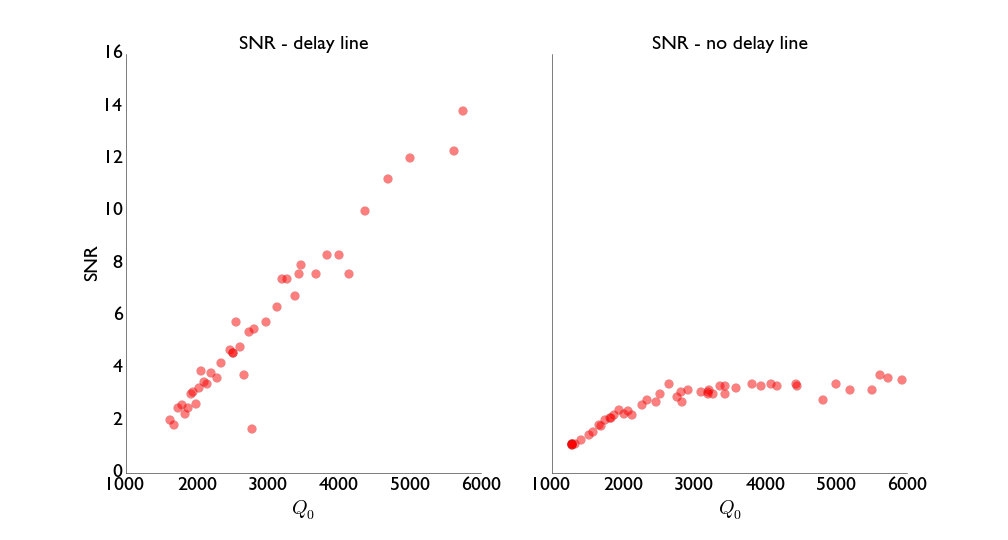
\includegraphics[width=\textwidth]{summary_plots}
\caption{}
\label{fig:summary_plots}
\end{figure}

\subsection{Comparison with Simulation}

\section{Discussion}

\section{Wild Speculation}

\section{Bibliography}

\end{document}  